\documentclass{amsart}
\usepackage{tikz}
\usepackage{float}

\usepackage{amsmath}
\usepackage{amsfonts}
\usepackage{amsthm}
\usepackage{enumitem}
\usepackage{dsfont}
\usepackage{amssymb}
\usepackage{pifont}
\usepackage{mathtools}

\newtheorem{thm}{Theorem}[section]
\newtheorem{lem}[thm]{Lemma}
\newtheorem{prop}[thm]{Proposition}
\newtheorem{conj}[thm]{Conjecture}
\newtheorem{cor}[thm]{Corollary}

\newtheorem*{prop*}{Proposition}

\theoremstyle{definition}
\newtheorem{claim}[thm]{Claim}
\newtheorem{defn}[thm]{Definition}
\newtheorem{quest}[thm]{Question}
\newtheorem{remark}[thm]{Remark}
\newtheorem{fact}[thm]{Fact}
\newtheorem{note}[thm]{Note}

\newtheorem*{claim*}{Claim}
\newtheorem*{quest*}{Question}
\newtheorem*{remark*}{Remark}
\newtheorem*{fact*}{Fact}

\newcommand{\N}{\ensuremath{\mathbb{N}}}
\newcommand{\Z}{\ensuremath{\mathbb{Z}}}
\newcommand{\Q}{\ensuremath{\mathbb{Q}}}
\newcommand{\R}{\ensuremath{\mathbb{R}}}
\newcommand{\C}{\ensuremath{\mathbb{C}}}
\newcommand{\F}{\ensuremath{\mathbb{F}}}
\newcommand{\AP}{\ensuremath{\mathcal{A}_{2^{n}}}}
\newcommand{\BP}{\ensuremath{\mathcal{B}_{2^{n}}}}
\newcommand{\CP}{\ensuremath{\mathcal{C}_{2^{n}}}}
\newcommand{\DP}{\ensuremath{\mathcal{D}_{2^{n}}}}
\newcommand{\EP}{\ensuremath{\mathcal{E}_{2^{n}}}}
\newcommand{\FP}{\ensuremath{\mathcal{F}_{2^{n}}}}

\newcommand{\E}{\ensuremath{\mathbb{E}}}
\newcommand{\1}{\ensuremath{\mathds{1}}}

\newcommand{\pair}[2]{\ensuremath{\langle #1, #2 \rangle}}

\DeclareMathOperator{\Gal}{Gal}
\DeclareMathOperator{\Jac}{Jac}
\DeclareMathOperator{\Var}{Var}
\DeclareMathOperator{\Cov}{Cov}
\DeclareMathOperator{\Div}{Div}
\DeclareMathOperator{\Prin}{Prin}        
\DeclareMathOperator{\im}{im}
\DeclareMathOperator{\val}{val}

\newcommand{\bv}[1]{\widehat{\mathbf{#1}}}
\renewcommand{\thefootnote}{\fnsymbol{footnote}}

\title{Jacobians of finite graphs and the monodromy pairing}
\author{Louis Gaudet, Nicholas Wawrykow, Theodore Weisman}

\begin{document}

\maketitle

Unless stated otherwise, we will take a ``graph'' to mean a finite
connected multigraph with no loops.

\section{Jacobians of Finite Graphs}
\label{sec:jacobians}

\subsection{The general graph case}
It is natural to ask which finite abelian groups appear as Jacobians
of graphs. The problem can be considerably reduced by the following
proposition:

\begin{prop}
\label{prop:wedge_product}
Let $G_1$ and $G_2$ be graphs. Then $\Jac(G_1 \vee G_2) \simeq
\Jac(G_1) \times \Jac(G_2)$.
\end{prop}

We prove Proposition \ref{prop:wedge_product} by observing that the
Jacobian of a graph can be directly computed from the Smith normal
form of its Laplacian matrix. Throughout the following, for any
integer matrix $M$, let $M_{i,i}$ represent the submatrix of $M$ obtained
by deleting the $i$th row and column.

\begin{lem}
\label{lem:SNF_submatrix}
Let $G$ be a graph, and let $Q$ be the Laplacian matrix of $G$. If the
Smith normal form of $Q$ is $S$, then for any $i$, the Smith normal
form of $Q_{i,i}$ is $S_{n,n}$.
\end{lem}
\begin{proof}
  WE NEED A PROOF OF THIS, but I feel like someone has to have proved
  it already so I'm not typing it.
\end{proof}

\begin{proof}[Proof of Proposition \ref{prop:wedge_product}]
  Let $Q_1$ and $Q_2$ be the Laplacian matrices of $G_1$ and $G_2$,
  respectively, and let the vertex of intersection of $G_1$ and $G_2$
  be $v_0$. Enumerate the vertices of $G$ so that the Laplacian of $G$
  can be written as
\begin{equation*}
  Q = 
  \left[\begin{array}{ccc}
      Q_1 & \vdots & \\
      \ldots & \val{v_0}  & \ldots \\
      & \vdots & Q_2
  \end{array}\right]
\end{equation*}
If we delete the row and column corresponding to $v_0$, the resulting
matrix $Q'$ will be in block diagonal form, and has cokernel
isomorphic to that of the matrix obtained by taking the Smith normal
form of the blocks. Applying Lemma \ref{lem:SNF_submatrix}, we then
see that the following matrix $M$ has cokernel isomorphic to the
cokernel of $Q$:

\begin{equation*}
  \left[\begin{array}{cc|c}
      S_1 & \\
      & S_2 \\ \hline
      & & 0
    \end{array}\right]
\end{equation*}

where $S_1$, $S_2$ are diagonal matrices whose entries are the
invariant factors of $\Jac(G_1), \Jac(G_2)$, respectively.
\end{proof}

\begin{figure}[h]
  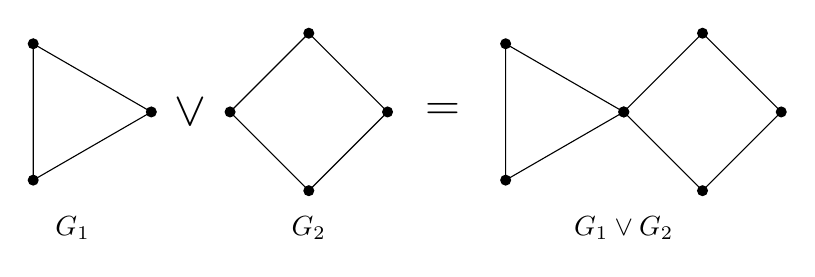
\begin{tikzpicture}

    
    \draw {(0:1) -- (120:1) -- (240:1)} -- cycle (270:1.2) node[below]
    {$G_1$};
    \foreach \theta in {0, 120, 240} {
      \fill (\theta:1) circle (2pt) ;
    } ;

    \node at (0:1.5) {\LARGE $\vee$};

    \begin{scope}[xshift=3cm]
      \draw {(0:1) -- (90:1) -- (180:1) -- (270:1)} -- cycle (270:1.2)
      node[below] {$G_2$};

      \foreach \theta in {0, 90, ...,  270} {
        \fill (\theta:1) circle (2pt) ;
      } ;
    \end{scope}

    \node at (0:4.7) {\LARGE $=$} ;

    \begin{scope}[xshift=6cm]
      \draw {(0:1) -- (120:1) -- (240:1)} -- cycle ;
      \foreach \theta in {0, 120, 240} {
        \fill (\theta:1) circle (2pt) ;
      } ;
      \begin{scope}[xshift=2cm]
        \draw {(0:1) -- (90:1) -- (180:1) -- (270:1)} -- cycle ;
        
        \foreach \theta in {0, 90, ...,  270} {
          \fill (\theta:1) circle (2pt) ;
        } ;
      \end{scope}
      \node[below] at (1,-1.2) {$G_1 \vee G_2$} ;
    \end{scope}
  \end{tikzpicture}
  \caption{The wedge sum operation on graphs. In this case, $\Jac(G_1)
  \simeq \Z/3\Z$, $\Jac(G_2) \simeq \Z/4\Z$, and $\Jac(G_1 \vee G_2)
  \simeq \Z/12\Z$.}
\end{figure}

Note that in the case that $G_1$ is a tree (and therefore $\Jac(G_1)$
is trivial), $\Jac(G_1 \vee G_2) \simeq \Jac(G_2)$. We then have
the following corollary:
\begin{cor}
  \label{cor:1_valent}
  Let $G$ be a graph, and let $A = \{v \in V(G) : \val(v) > 1\}$. If
  $G'$ is the subgraph of $G$ induced by $A$, then $\Jac(G) \simeq
  \Jac(G')$.
\end{cor}

Proposition \ref{prop:wedge_product}, together with the classification
theorem for finite abelian groups, tells us that if, for all $n$,
there exists a graph $G$ such that $\Jac(G)$ is cyclic of order $n$,
then \emph{all} finite abelian groups are the Jacobian of some graph.

For given $n$, we give two possible constructions of $G$ with $\Jac(G)
\simeq \Z/n\Z$.

\begin{defn}
  $B_n$, the \emph{banana graph on $n$ edges}, is the graph with
  $V(B_n) = \{v_1, v_2\}$ and edge multiset consisting of $n$ copies of
  $\{v_1, v_2\}$.
\end{defn}

\begin{figure}[h]
  \begin{center}
    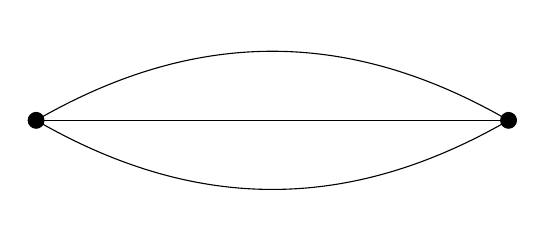
\begin{tikzpicture}
      \draw (0,0) to [out=30, in=150] (6,0) ;
      \draw (0,0) to [out=-30, in=-150] (6,0) ;
      \draw (0,0) to [out=0, in=180] (6,0) ;

      \draw [fill] (0,0) circle [radius=.1cm] ;
      \draw [fill] (6,0) circle [radius=.1cm] ;      
    \end{tikzpicture}
    \caption{The $3$-banana $B_3$}
  \end{center}
\end{figure}

\begin{prop}
  \label{prop:banana_cyclic}
  Let $B_n$ be the banana graph on $n$ edges. Then $\Jac(B_n) \simeq \Z/n\Z$.
\end{prop}

\begin{proof}
  $B_n$ has $n$ spanning trees, so
  $|\Jac(B_n)| = n$. To show that $\Jac(B_n) \simeq \Z/n\Z$, it
  suffices to find a single element of order at least $n$.

  Let $D \in \Div^0(B_n)$ be the divisor $(v_2) - (v_1)$, and consider
  $\overline{D} = [D] \in \Jac(B_n)$. For any $1 \le m < n$, the
  divisor $mD$ is $v_1$-reduced---since $v_2$ has degree $n$, it is
  impossible to fire it without sending it into debt. If $m=n$, then
  firing $v_2$ yields the zero divisor. $m\overline{D}$ is therefore
  trivial iff $m$ is a multiple of $n$, and hence $\overline{D}$ has
  order $n$ as required.
\end{proof}

\subsection{The simple graph case}
The construction given above is sufficient to show that all finite
abelian groups appear as the Jacobian of some graph. However, since
banana graphs are only realizable as a multigraphs, we might also wish
to find a construction for a simple graph $G$ with $\Jac(G) \simeq
\Z/n\Z$ for given $n$. This is (almost) always possible, by the
following proposition:

\begin{prop}
  \label{prop:cycle_cyclic}
  Let $C_n$ be the cycle graph on $n \ge 2$ vertices. Then $\Jac(C_n) \simeq
  \Z/n\Z$.
\end{prop}

$C_n$ has $n$ spanning trees, so $|\Jac(C_n)|=n$ and, as before, it
suffices to find a single element of $\Jac(C_n)$ of order at least
$n$. With the following lemma, we show that such an element exists on a wider family of graphs:

\begin{lem}
  \label{lem:2valent_path}
  Let $G$ be a biconnected graph, and suppose that for some path $P =
  \{v_1, \ldots, v_\ell\}$ on $G$, $\val(v_i) = 2$ for all $1 < i <
  \ell$. Then $\Jac(G)$ contains an element of order at least $\ell$.
\end{lem}
\begin{proof}
  Consider the divisor $D = (v_2) - (v_1)$. We claim that for any $1
  \le m < \ell$, $mD$ is equivalent to $(v_{m+1}) - (v_1)$.

  I'm going to make either a chip-firing argument or a Laplacian
  matrix argument for why this is true, but it's pretty cumbersome so
  I'll leave it for later.

  $G$ is biconnected, so there is a path from $v_1$ to $v_{m+1}$ that
  does not contain any vertex $v_i$ for $1 < i < m$. Applying the
  burning algorithm then shows that the divisor $(v_{m+1}) - (v_1)$ is
  $v_1$-reduced, and hence $m\overline{D} = m[D]$ is nontrivial for $m
  < \ell$, as required.
\end{proof}

$C_n$ is a simple graph whenever $n > 2$, so we have the following:

\begin{cor}
  Let $\Gamma$ be a finite abelian group that is not isomorphic to
  $\Z/2\Z \times H$ for any group $H$. Then there exists a simple
  graph $G$ such that $\Gamma \simeq \Jac(G)$.
\end{cor}

The rest of this section will investigate which groups $\Gamma =
\Z/2\Z \times H$ can possibly occur as the Jacobian of some simple
graph. It is known that there is no simple graph $G$ with $\Jac(G)
\simeq \Z/2\Z$, since there is no simple graph with two spanning trees. We extend this result as
follows:

\begin{thm}
  \label{thm:2group}
  For any $k \ge 1$, if $G$ is a graph such that $\Jac(G) \simeq
  (\Z/2\Z)^k$, then $G$ is not simple.
\end{thm}

\begin{thm}
  \label{thm:2group_product}
  Let $H$ be a finite abelian group. There exists an integer $k_0$
  (depending only on $H$) such that for all $k > k_0$, there does not exist
  a simple graph $G$ with $\Jac(G) \simeq (\Z/2\Z)^k \times H$.
\end{thm}

To prove Theorem \ref{thm:2group_product}, we will first prove it in the case
where $G$ is biconnected. If $G$ is a
graph that is not biconnected, then by definition, there is a vertex
$v_0$ such that the subgraph $G'$ induced by $V(G) \setminus \{v_0\}$
is not connected. $G$ is then the wedge sum of the connected components of
$G'$ (together with the vertex $v_0$), and so $\Jac(G)$ breaks down as
a direct product of Jacobians of subgraphs of $G$.

\begin{defn}
  Let $G$ be a graph, and let $\Gamma = \Jac(G)$. We will write $\mu(G)$
  for the maximum order of an element of $\Gamma$, and $\delta(G)$ for
  the maximum valency of a vertex in $G$. (When the graph $G$ is clear
  from context, we will simply write $\delta$ or $\mu$). 
\end{defn}

\begin{lem}
  \label{lem:delta_le_mu}
  If $G$ is biconnected, then $\delta \le \mu$.
\end{lem}
\begin{proof}
  Let $v$ be a vertex in $V(G)$ with valency $\delta$, and let $w$ be
  a vertex adjacent to $w$. Consider the divisor $D = (v) -
  (w)$, and let $m < \delta$ be a positive integer. 

  We may apply Dhar's burning algorithm to check that $mD$ is
  $w$-reduced. Since $G$ is biconnected, there is a path from $w$ to
  each of the neighbors of $v$ that does not contain $v$, and so each
  of the neighbors of $v$ is burned during the algorithm. $v$ has more
  than $m$ distinct neighbors, so it is burned as well. Therefore,
  $m\overline{D}$ is nontrivial and $\overline{D}$ has order at least
  $\delta$.
\end{proof}

\begin{cor}
  \label{cor:genus_v_mu}
  For any biconnected graph with genus $g$ and $|V(G)| = v$,
  \begin{equation*}
    v \ge \frac{2g - 2}{\mu - 1}.
  \end{equation*}
\end{cor}
\begin{proof}
  Let $e = |E(G)|$. We have 
  \begin{equation*}
    2e = \sum_{i=1}^n \val(v_i) \le \sum_{i=1}^n \delta = v \cdot \delta
    \le v \cdot \mu.
  \end{equation*}
  Since $e = g + v - 1$, this gives $2g - 2 \le v \cdot (\mu - 1)$, as required.
\end{proof}

\begin{proof}[Proof of Theorem \ref{thm:2group}]
  Let $G$ be a biconnected graph with $\Jac(G) = (\Z/2\Z)^k$. By
  Corollary \ref{cor:1_valent}, we may assume without loss of
  generality that each vertex of $G$ has valency at least $2$. By
  Lemma \ref{lem:delta_le_mu}, each vertex of $G$ has valency exactly
  $2$, hence $G = C_n$ for some $n$. We must have $n=2$, which means $G$
  cannot be simple.

  Now let $G$ be a graph that is not biconnected, with $\Jac(G) \simeq
  (\Z/2\Z)^k$. We proceed by induction on $k$.
  
  The base case $k=1$ is known. For $k > 1$, note that $\Jac(G) \simeq
  \Jac(G_1) \times \Jac(G_2)$ for connected subgraphs $G_1, G_2$ of
  $G$. Without loss of generality, $G_2$ is not a tree, and
  hence $\Jac(G_1) \simeq (\Z/2\Z)^{k_1}$ for $k_1 < k$. By the
  induction hypothesis, $G_1$ is not simple, and so neither is $G$.
\end{proof}

\begin{remark}
  The proof of Theorem \ref{thm:2group} also gives a complete
  characterization of any graph $G$ with $\Jac(G) \simeq
  (\Z/2\Z)^k$: in general, $G$ must be a tree with precisely $k$ of
  the edges occuring two times. We will apply this fact later, in our
  discussion of the monodromy pairing on $\Jac(G)$.
\end{remark}

\begin{figure}[H]
  \begin{center}
    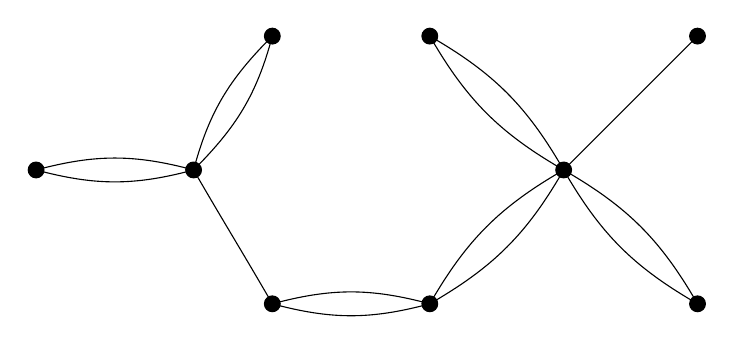
\begin{tikzpicture}

      \draw (0,0) to [out=15, in=165] (2,0) ;
      \draw (0,0) to [out=-15, in=-165] (2,0) ;

      \draw (2,0) to [out=75, in=225] (3, 1.7) ;
      \draw (2,0) to [out=45, in=255] (3, 1.7) ;

      \draw (2,0) to [out=-60, in=-240] (3, -1.7) ;

      \draw (3,-1.7) to [out=15, in=165] (5, -1.7) ;
      \draw (3,-1.7) to [out=-15, in=-165] (5, -1.7) ;

      \draw (5, -1.7) [out=60, in=210] to (6.7, 0) ;
      \draw (5, -1.7) [out=30, in=240] to (6.7, 0) ;

      \draw (6.7, 0) [out=120, in=-30] to (5, 1.7) ;
      \draw (6.7, 0) [out=150, in=-60] to (5, 1.7) ;

      \draw (6.7, 0) to (8.4, 1.7) ;

      \draw (6.7, 0) to [out=-30, in=120] (8.4, -1.7) ;
      \draw (6.7, 0) to [out=-60, in=150] (8.4, -1.7) ;

      \draw [fill] (0,0) circle [radius=.1cm] ;
      \draw [fill] (2,0) circle [radius=.1cm] ;
      \draw [fill] (3,1.7) circle [radius=.1cm] ;
      \draw [fill] (3,-1.7) circle [radius=.1cm] ;
      \draw [fill] (5,-1.7) circle [radius=.1cm] ;
      \draw [fill] (6.7, 0) circle [radius=.1cm] ;
      \draw [fill] (5,1.7) circle [radius=.1cm] ;
      \draw [fill] (8.4,1.7) circle [radius=.1cm] ;
      \draw [fill] (8.4,-1.7) circle [radius=.1cm] ;
    \end{tikzpicture}
    \caption{$\Jac(G) \simeq (\Z/2\Z)^6$}
  \end{center}
\end{figure}

We will now prove Theorem \ref{thm:2group_product}, using a similar
inductive argument on biconnected subgraphs. Throughout the following,
we will suppose that $G$ is a biconnected graph with Jacobian $\Gamma
\simeq (\Z/2\Z)^k \times H$ for some finite abelian group $H$, and
that $\mu$ is the maximum order of an element of $H$. We first
establish a bound on the genus of $G$:

\begin{lem}
  \label{lem:genus_cycle}
  If $g$ is the genus of $G$, then $g \ge k$.
\end{lem}
\begin{proof}
  For any graph $G_0$, let $h(G_0)$ be the number of nontrivial invariant
  factors of $\Jac(G_0)$. Let $G_0'$ be the graph obtained by adding a
  single edge to $G_0$. We know $|h(G_0') - h(G_0)| \le 1$ (CITE
  THIS). 
%%%%%%%%%%%%%%%%%%%%%%%%%%%%%%%%%%%%%%%%%%%%%%%%%%%%%%%%%%%%%%%%%%%%%%%%%%%%%%%%%%%%%%%%

  Since a graph $G$ with genus $g$ may be constructed by adding $g$ edges
  to a spanning tree for $G$, $\Jac(G)$ has at most $g$ invariant
  factors, and thus at most $g$ factors of $\Z/2\Z$. 
\end{proof}

Applying Corollary \ref{cor:genus_v_mu} to this result gives us a
lower bound on $|V(G)|$ in terms of $k$ and $\mu$. We now establish an
upper bound on $|V(G)|$ in terms of $\mu$ and $|H|$, to achieve an
upper bound on $g$, and hence $k$.

\begin{prop}
  \label{prop:v_bound}
  Suppose that $G$ is biconnected. Then for any finite abelian group $H$, there exists an integer $v_0$
  (depending only on $H$) such that if $\Gamma = \Jac(G) \simeq (\Z/2\Z)^k
  \times H$, then $|V(G)| < v_0$.
\end{prop}

\begin{proof}
  Let $U = \{u \in V(G) : \val(u) > 2\}$, and enumerate the elements
  of $U$ as $u_1, \ldots, u_m$. We will first establish a bound on
  $m = |U|$, and then bound $|V(G)|$ in terms of $m$.
  
  Consider the set of divisors $\mathcal{U} = \{(u_i) - (u_1) : 1 \le
  i \le m\}$, and let $\overline{\mathcal{U}} \subseteq \Gamma$ be the set of equivalence
  classes of the elements of $\mathcal{U}$. Write $D_i$ for $(u_i) - (u_1)$. For any $D_i, D_j \in
  \mathcal{U}$, we claim that $2D_j - 2D_i$ is $u_i$-reduced.

  We have $2D_j - 2D_i = 2(u_j) - 2(u_i)$. Since $G$ is biconnected,
  there is a path from $u_i$ to each of the neighbors of $u_j$ that
  does not contain $u_j$. Since $u_j$ has valency at least $3$, an
  iteration of the burning algorithm must burn $u_j$, and in turn the
  entire graph. Furthermore, since $2D_j - 2D_i$ is $u_i$-reduced,
  $2[D_j] \ne 2[D_i]$ for any $i \ne j$. Note that this also implies that
  $[D_j] \ne [D_i]$ for any $i \ne j$, so we have $m=|\overline{\mathcal{U}}|$. 

  Now let $\phi:\Gamma \to \Gamma$ be the map given by
  \[
  \phi(\overline{D}) = 2\overline{D}.
  \] 

  By the above, we have $|\phi(\overline{\mathcal{U}})|=|\overline{\mathcal{U}}|=m$. Further $|\im(\phi)| \le |H|$, and so 
  we get $m=|\phi(\overline{\mathcal{U}})| \le |H|$, as desired.

  We now wish to bound $|V(G)|$ in terms of $m$. To do so, we will
  consider a graph $G'$, given by the following transformation of $G$:

  \begin{enumerate}
  \item Choose some vertex of $G$ of valency $2$. Delete it, and
    draw an edge between its neighbors.
  \item Repeat until there are no 2-valent vertices remaining.
  \end{enumerate}
  %%%%%%%%%%%%%%%%%%%%%%%%%%%%%%%%%%%%%%%%%%%%%%%%%%%%%%%%%%%%%%%%%%%%%%%%%%%%%%%%%%%%%%%% 

  \begin{figure}[H]
    \begin{center}
      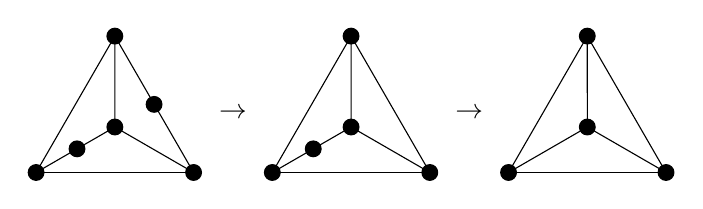
\begin{tikzpicture}

        \draw (0:0) to (60:2) ;
        \draw (0:0) to (0:2) ;
        \draw (60:2) to (0:2) ;
        \draw (0:0) to (30:1.155) ;
        \draw (0:2) to (30:1.155) ;
        \draw (60:2) to (30:1.155) ;

        \draw [fill] (0:0) circle [radius=.1cm] ;
        \draw [fill] (0:2) circle [radius=.1cm] ;
        \draw [fill] (60:2) circle [radius=.1cm] ;
        \draw [fill] (30:1.155) circle [radius=.1cm] ;
        \draw [fill] (30:.6) circle [radius=.1cm] ;
        \draw [fill] (30:1.73) circle [radius=.1cm] ;

        \draw [shift={(3,0)}] (0:0) to (60:2) ;
        \draw [shift={(3,0)}] (0:0) to (0:2) ;
        \draw [shift={(3,0)}] (60:2) to (0:2) ;
        \draw [shift={(3,0)}] (0:0) to (30:1.155) ;
        \draw [shift={(3,0)}] (0:2) to (30:1.155) ;
        \draw [shift={(3,0)}] (60:2) to (30:1.155) ;

        \draw [shift={(3,0)}][fill] (0:0) circle [radius=.1cm] ;
        \draw [shift={(3,0)}][fill] (0:2) circle [radius=.1cm] ;
        \draw [shift={(3,0)}][fill] (60:2) circle [radius=.1cm] ;
        \draw [shift={(3,0)}][fill] (30:1.155) circle [radius=.1cm] ;
        \draw [shift={(3,0)}][fill] (30:.6) circle [radius=.1cm] ;

        \draw [shift={(6,0)}] (0:0) to (60:2) ;
        \draw [shift={(6,0)}](0:0) to (0:2) ;
        \draw [shift={(6,0)}](60:2) to (0:2) ;
        \draw [shift={(6,0)}](0:0) to (30:1.155) ;
        \draw [shift={(6,0)}](0:2) to (30:1.155) ;
        \draw [shift={(6,0)}](60:2) to (30:1.155) ;

        \draw [shift={(6,0)}][fill] (0:0) circle [radius=.1cm] ;
        \draw [shift={(6,0)}][fill] (0:2) circle [radius=.1cm] ;
        \draw [shift={(6,0)}][fill] (60:2) circle [radius=.1cm] ;
        \draw [shift={(6,0)}][fill] (30:1.155) circle [radius=.1cm] ;

        \node at (2.5, .75) {$\rightarrow$} ;
        \node at (5.5, .75) {$\rightarrow$} ;

      \end{tikzpicture}
      \caption{The transformation $G \mapsto G'$}
    \end{center}
  \end{figure}

  Note that even if $G$ is simple, $G'$ need not be. It is clear,
  however, that $G$ and $G'$ have the same number of vertices with
  valency greater than $2$, and that $\delta(G) = \delta(G')$.

  By Lemma \ref{lem:delta_le_mu}, we must have that $e' = |E(G')|$ is
  at most $m \cdot \mu$ (since otherwise there would necessarily be a
  vertex of $G$ with valency greater than $\delta$). Each 2-valent
  vertex of $G$ is uniquely associated with some edge of $G'$. If
  there are more than $e' \cdot \mu$ 2-valent vertices in $G$, then at
  least $\mu$ of them are associated with a single edge of $G'$. 

  In this case, $G$ would contain a path $P$ of length greater than $\mu$, where
  each vertex of $P$ has valency $2$. This would contradict Lemma
  \ref{lem:2valent_path}, so instead we have 
  \[
  |V(G)| - m < m\mu^2.
  \] 
  Choosing $v_0 = |H|(1 + \mu^2)$ then gives $|V(G)| < v_0$, as
  required.
\end{proof}

Applying Corollary \ref{cor:genus_v_mu} and Lemma
\ref{lem:genus_cycle}, we see that for sufficiently large $k$, we must
have $|V(G)| > v_0$. This in turn implies that for sufficiently large
$k$, $(\Z/2\Z)^k \times H$ is not the Jacobian of any biconnected
graph.

We now complete the proof of Theorem \ref{thm:2group_product} via
induction on $|H|$.
  
\begin{proof}[Proof of Theorem \ref{thm:2group_product}]
When $|H| = 1$ or $2$, Theorem \ref{thm:2group} gives the
bound $k_0 = 1$. For $|H| \ge 3$, there must exist (by Proposition
\ref{prop:v_bound}) an integer $k'$ such that if $k > k'$, and
$\Jac(G) \simeq (\Z/2\Z)^k \times H$, then $G$ is not biconnected.

By the induction hypothesis, for any proper subgroup $H' \subset H$,
there exists an integer $k(H')$ such that for all $k > k(H')$, no
simple graph $G'$ has $\Jac(G') \simeq (\Z/2\Z)^k \times H'$. Now,
since $H$ is finite, there are finitely many pairs of nontrivial
proper subgroups $H_1, H_2 \subset H$ such that $H_1 \times H_2 \simeq
H$. Define

\begin{equation*}
  k'' = \max\{k(H_1) + k(H_2) : H_1, H_2 \textrm{ nontrivial}, H_1
  \times H_2 \simeq H\}
\end{equation*}

Now let $k_0 = \max(k', k'')$. We wish to show that for all $k > k_0$,
if $\Jac(G) \simeq (\Z/2\Z)^k \times H$, then $G$ is not simple. Let
$G$ be a graph with this Jacobian, and let $k > k_0$.  Since $k > k'$,
$G$ is not biconnected, so it must be the wedge sum of two graphs
$G_1$ and $G_2$. There must then exist integers $k_1, k_2$ with $k_1 +
k_2 = k$ and groups $H_1, H_2$ with $H_1 \times H_2 \simeq H$ such
that

\begin{align}
  \Jac(G_1) &\simeq (\Z/2\Z)^{k_1} \times H_1 \\
  \Jac(G_2) &\simeq (\Z/2\Z)^{k_2} \times H_2
\end{align}

Without loss of generality, we may assume that neither $G_1$ nor $G_2$
is a tree, so that $\Jac(G_1)$ and $\Jac(G_2)$ are both nontrivial. In
that case, if either $H_1$ or $H_2$ were trivial, then $G_1$
(resp. $G_2$) would have Jacobian isomorphic to $(\Z/2\Z)^k$ for $k >
0$, implying that at least one of $G_1$ or $G_2$ is not simple.

Finally, since $k_1 + k_2 = k > k'' \ge k(H_1) + k(H_2)$, we must have
that either $k_1 > k(H_1)$ or $k_2 > k(H_2)$. Then either $G_1$ or
$G_2$ is not simple, so that $G$ is not simple, as required.
\end{proof}

\subsection{Further queries} 

Analysis of the proof of Theorem \ref{thm:2group_product} suggests
that, if $H$ is cyclic of prime power order, $k_0(H)$ is
$O(|H|^4)$. In practice, it seems that much better bounds should
hold. For instance, no simple graph $G$ has yet been found where
$\Jac(G) \simeq (\Z/2\Z)^k \times H$ for any $k > |H|$.

In some cases, it is possible to directly verify that certain groups
do not arise as the Jacobian of any simple graph. We note that, for
given $m$, while there are infinitely many isomorphism classes of
simple graphs with fewer than $m$ spanning trees, at most finitely
many of these classes represent 2-edge-connected graphs. (THIS MIGHT
NEED A PROOF).

Lemma \ref{prop:wedge_product} tells us that any graph $G$ may be
uniquely associated to some 2-edge-connected graph with identical
Jacobian. For a given group $H$, it is possible to compute the
Jacobian of all 2-edge-connected simple graphs with at most $|H|$
spanning trees, and verify that $H$ does or does not occur. 

Computer searches of this nature have led to the following:

\begin{thm}
  The groups $\Z/2\Z \times \Z/4\Z$, $(\Z/2\Z)^2 \times \Z/4\Z$, and
  $\Z/2\Z \times (\Z/4\Z)^2$ are not isomorphic to the Jacobian of any
  simple graph.
\end{thm}

It is also of interest that the key fact in the proof of the
nonoccurence of groups with many factors of $\Z/2\Z$ seems to be the
requirement that $G$ is biconnected, rather than that $G$ is
simple. This, together with the discovery that the Jacobians of
``most'' graphs are cyclic (CITE STUFF), suggests the following:

\begin{conj}
  Let $G$ be a biconnected graph. For any $n$, there exists $k_0$ such
  that if $k > k_0$, $\Jac(G) \not\simeq (\Z/n\Z)^k$.
\end{conj}

Finally, we note that when $\Jac(G) \simeq (\Z/n\Z)^k \times H$ for
some finite abelian group $H$, $k$ is necessarily bounded above by the
genus of $G$. The next section will consider certain circumstances
under which this bound can be achieved, and also say some things about
metric graphs.

\section{Relationship to Jacobians of Metric Graphs}
\begin{lem}
  \label{lem:jac_generators}
  Let $G$ be a graph. $\Jac(G)$ is generated by the set \[\{[(v) -
  (w)]: \{v, w\} \in E(G)\}\]
\end{lem}

\begin{proof}
  In general, $\Div^0(G)$ is generated by divisors of the form $(v_a)
  - (v_b)$ for $v_a, v_b \in V(G)$. Since $G$ is connected, any such
  divisor may be represented as a sum of divisors of the form $(v) -
  (w)$ for adjacent $v$ and $w$ (formal proof can be given if
  necessary). Therefore the Jacobian is generated by the equivalence
  classes of these divisors.  
\end{proof}

\section{The monodromy pairing on the Jacobian}


The Jacobian of a finite graph is endowed with a natural monodromy
pairing. Since it is possible to classify all finite abelian groups
with pairing, it is worth considering which groups \emph{with pairing}
occur as the Jacobian of some graph. This section will investigate
this question.

\begin{note}
  Throughout the following, unless otherwise noted, we will always use
  the word ``group'' to mean ``group \emph{with pairing},''
  ``isomorphism'' and ``$\simeq$'' to mean an isomorphism of groups
  with pairing, and $\oplus$ to denote the orthogonal sum on groups
  with pairing. For a graph $G$, we will take $\Jac(G)$ to mean the
  Jacobian of $G$ with its associated monodromy pairing.
\end{note}

Our main result will be the following:

\begin{thm}
  \label{thm:graph_pairing}
  Let $\Gamma$ be a finite abelian group of odd order, not isomorphic
  to $(\Z/p\Z) \times H$ for any prime $p \equiv 1 \pmod {24}$ and
  group $H$. Then there exists a graph $G$ such that
  \[
  \Jac(G) \simeq \Gamma
  \]
\end{thm}

\subsection{Basic constructions}

As in the case of groups without pairing, we will take advantage of
the fact that the wedge sum of two graphs corresponds to a product
operation on the Jacobians of those graphs. In this case, the
``product'' will be the orthogonal sum:

\begin{prop}
  \label{prop:wedge_sum}
  Let $G_1$, $G_2$ be graphs. Then $\Jac(G_1 \vee G_2) \simeq
  \Jac(G_1) \oplus \Jac(G_2)$. 
\end{prop}
\begin{proof}
  DANIEL MITROPOLSKY WHY HAVE YOU FORSAKEN US
\end{proof}

The problem is now reduced to the following: given a prime $p$, a
positive integer $r$, and a pairing $\pair{\cdot}{\cdot}$ on
$\Z/p^r\Z$, we wish to find a graphs $G$ such that $\Jac(G) \simeq
(\Z/p^r\Z, \pair{\cdot}{\cdot})$.

Section \ref{sec:jacobians} gave a construction for graphs with any
desired Jacobian, but we require a way to construct graphs whose
Jacobian is associated with a particular pairing. We provide two
possible constructions below:

\begin{defn}
  Let $S = \{s_1, \ldots, s_m\}$ be a multiset of positive
  integers. $B_S$, the \emph{subdivided banana graph of $S$}, is the
  graph obtained by subidividing the $i$th edge of $B_m$ by $s_i-1$
  vertices.
\end{defn}

\begin{defn}
  Let $S = \{s_1, \ldots, s_m\}$ be a multiset of positive
  integers. $C_S$, the \emph{stupidly named cycle graph of $S$}, is
  the graph obtained giving the $i$th edge of $C_m$ multiplicity
  $s_i$.
\end{defn}

When $|S| = m$, we will use the following notation for the $(m-1)$th
elementary symmetric polynomial applied to the elements of $S$:

\begin{defn}
  Let $S = \{s_1, \ldots, s_m\}$. Define
  \begin{align*}
    R(S) &= \sum_{i=1}^m\frac{\prod_{j=1}^ms_j}{s_i}
  \end{align*}
\end{defn}

\begin{prop}
  \label{prop:banana_pairing}
  Let $S$ be a multiset of positive integers such that $R(S) = p^r$
  for a prime $p$ and integer $r$, and $\gcd(s_i, p) = 1$ for all $s_i
  \in S$. Then
  \begin{equation*}
    \Jac(B_S) \simeq (\Z/p^r\Z, \pair{\cdot}{\cdot})
  \end{equation*}
  where $\pair{\cdot}{\cdot}$ is the pairing on $\Z/p^r\Z$ given by
  \begin{equation*}
    \pair{x}{y} = \frac{\left(\prod_{i=1}^ms_i\right)xy}{p^r}
  \end{equation*}
\end{prop}
\begin{proof}
  We first show that $|\Jac(B_S)| = p^r$. Let $|S| = m$. We may
  partition the edges of $B_S$ into sets $E_1, \ldots, E_m$, where
  $E_i$ corresponds to the $i$th edge of the banana graph $B_m$. The
  edge set of any spanning tree on $B_S$ must be

  \begin{equation*}
    E_i \cup \left(\bigcup_{j \ne i} (E_j \setminus \{e_{jk}\})\right)
  \end{equation*}
  where $e_{jk}$ is some edge in $E_j$. Each possible choice of $E_i$
  and $e_{jk}$ corresponds to a distinct spanning tree of $B_S$, so we
  have $R(S)$ spanning trees, as required.

  We will enumerate the vertices of $B_S$ as follows: let $v_0, v_0'$
  be the vertices corresponding to $v_1, v_2$ on $B_m$, and let
  $v_{ij}$ be the $j$th vertex that subdivides the $i$th edge of
  $B_m$.

  Now consider the divisor $D = (v_0') - (v_0)$. We claim that
  $m\overline{D} = m[D]$ is nontrivial for any $m < p^r$. Suppose
  otherwise, so that $p^tD$ is principal for $t < r$, and let $\Delta$
  be the Laplacian map of $G$. There must exist a function $f:V(G) \to
  \Z$ such that $\Delta f = D$.

  For each edge $e = \{u, v\} \in E(B_S)$, let $b(e) = f(u) - f(v)$
  (orient each edge to point from $v_{ij}$ to $v_{ij+1}$). Since $D(v)
  = 0$ for any $v \in V(G) \setminus \{v_0, v_0'\}$, we must have
  $b(e_1) = b(e_2)$ for any $e_1, e_2 \in E_i$.  If $a_i = b(e)$ for
  any $e \in E_i$, then the following conditions must both hold:
  
  \begin{enumerate}
    \item 
      \[
      \sum_{i=0}^m a_i = p^t
      \]
    \item
      \[
      a_is_i = f(v_2) \textrm{ for all } 1 \le i \le m
      \]
  \end{enumerate}

  Taking these conditions together with the fact that $R(S) = p^r$, we
  see
  \begin{equation*}
    p^t = \sum_{i=1}^m \frac{f(v_2)}{s_i^{-1}} = 
    \frac{f(v_2) p^r}{\prod_{i=1}^ms_i}
  \end{equation*}
  \begin{equation*}
    \prod_{i=1}^ms_i = p^{r-t}f(v)
  \end{equation*}
  For $r > t$, this is impossible, and thus the group is cyclic,
  generated by $\overline{D}$. 

  The monodromy pairing on $\Jac(B_S)$ is then entirely determined by
  the value of $\pair{\overline{D}}{\overline{D}}$. Consider the
  following function $f:V(G) \to \Z$:

  \begin{equation*}
    f(v) = 
    \begin{cases}
      0, & v = v_0 \\
      \prod_{i=1}^ms_i, & v = v_0' \\
      j \cdot s_i^{-1}\prod_{k=1}^ms_k, & v = v_{ij}
    \end{cases}
  \end{equation*}

  It is clear that $\Delta(f) = p^rD$, and hence that
  $\pair{\overline{D}}{\overline{D}} = \frac{\prod_{i=1}^ms_i}{p^r}$.
\end{proof}

The cycle graph $C_n$ and the banana graph $B_n$ are both special
cases of the subdivided banana. As a result, we have:

\begin{cor}
  For any prime $p$ and integer $r$, 
  \begin{equation*}
    \Jac(B_{p^r}) \simeq (\Z/p^r\Z, \pair{\cdot}{\cdot}_1)
  \end{equation*}
  \begin{equation*}
    \Jac(C_{p^r}) \simeq (\Z/p^r\Z, \pair{\cdot}{\cdot}_2)
  \end{equation*}
  where $\pair{\cdot}{\cdot}_1$ and $\pair{\cdot}{\cdot}_2$ are the
  pairings on $\Z/p^r\Z$ given by
  \begin{equation*}
    \pair{x}{y}_1 = \frac{xy}{p^r} \qquad \pair{x}{y}_2 = \frac{(-1)xy}{p^r}
  \end{equation*}
\end{cor}

\subsection{Groups of odd order}
\label{sec:odd_groups}

Our goal is to use the construction above to build graphs whose
Jacobian is isomorphic to $(\Z/p^r\Z, \pair{\cdot}{\cdot})$ for any
pairing $\pair{\cdot}{\cdot}$. We will first address the simpler
situation, where $p$ is odd. In this case, up to isomorphism, there
are only two pairings on $\Z/p^r\Z$; we will denote these by
$\mathfrak{r}$ and $\mathfrak{n}$, the \emph{residue} and
\emph{nonresidue} pairings, respectively. We will also assume that $r
> 1$, and discuss the $r=1$ case separately. 

We can see immediately that the banana graph $B_{p^r}$ always gives
rise to the residue pairing on $\Z/p^r\Z$. To achieve the nonresidue
pairing, it suffices to prove the following:

\begin{claim}
  \label{claim:exist_decomp}
  For any odd prime $p$ and integer $r > 1$, there exists a
  multiset of positive integers $S = \{s_1, \ldots s_m\}$ such that
  $R(S) = p^r$, $\gcd(p, s_i) = 1$ for all $i$, and $\prod_{i=1}^ms_i$
  is a nonresidue modulo $p$.
\end{claim}

We will need the following proposition, which follows from (CITATION):
\begin{prop}
  \label{prop:q_bound}
  For any prime $p$ and integer $r > 1$, there exists a prime
  quadratic nonresidue $q$ such that $q^2/4<p^r$, with $q\equiv 3\pmod
  4$ if $r$ is odd and $q\equiv 1\pmod 4$ if $r$ is even.
\end{prop}

\begin{lem}
  \label{lem:decompose_q_non}
  Let $q$ be a prime with $q \equiv 3 \pmod 4$. Then for any $k$
  with $\left( \frac{k}{q} \right) = -1$, there exists $0 < a < q$
  such that $a(q-a) \equiv k \pmod q$. 
\end{lem}
\begin{proof}
  Let the set of nonresidues modulo $q$ be $R_q$. Consider the map
  $\phi:\F_q \to \F_q$ given by $\phi(x) = -x^2$. The image of
  $\phi$ is a subset of $R_q$, since (by quadratic reciprocity)
  $-1$ is a nonresidue modulo $q$. Furthermore, since the polynomial
  $-x^2 - a$ has at most two roots in $\F_q$ (for any $a$), and
  $|R_q| = (q - 1)/2$, $\phi_k$ is onto $R_q$. 

  Since $k \in R_q$, choose $a$ such that $\phi(a) = k$, and note
  that $k \equiv -a^2 \equiv a(q-a) \pmod q$, as required.
\end{proof}
\begin{lem}
  \label{lem:decompose_q_res}
  Let $q$ be a prime with $q \equiv 1 \pmod 4$. Then for any $k$
  with $\left( \frac{k}{q} \right) = 1$, there exists $0 < a < q$
  such that $a(q-a) \equiv k \pmod q$.
\end{lem}
\begin{proof}
  Define $\phi$ as in Lemma \ref{lem:decompose_q_non}, and note that in
  this case quadratic reciprocity implies that $\phi$ is onto the set
  of residues modulo $q$ (since $-1$ is a residue mod $q$). $k$ is
  again in the image of $\phi$, so its decomposition can be
  constructed as before.
\end{proof}

\begin{lem}
  \label{lem:exist_q}
  Let $p$ be a prime with $p \equiv 1 \pmod 4$, and let $r$ be an
  integer with $r > 1$. Then there exists a prime $q$, with $\left(
    \frac{q}{p^r} \right) = -1$, and an integer $0 < a < q$ such that
  the quantity
  \[\frac{p^r - a(q-a)}{q}\] 
  is a positive integer.
\end{lem}
\begin{proof}
  First suppose $r$ is odd. By Proposition \ref{prop:q_bound}, there
  exists a prime $q \equiv 3 \pmod 4$ such that $\left( \frac{q}{p}
  \right) = -1$ and $\frac{q^2}{4} < p^r$.

  Since $r$ is odd, and $p \equiv 1 \pmod 4$, $p^r$ is a nonresidue
  modulo $q$. Apply Lemma \ref{lem:decompose_q_non} to find $a$ such
  that $p^r \equiv a(q-a) \pmod q$. Since $q < p$ and $r > 1$,
  $a(q-a) < p^r$. Therefore $p^r - a(q-a)$ is positive and divisible
  by $q$, as required.

  Now suppose $r$ is even. By Proposition \ref{prop:q_bound}, there
  exists a prime $q$ with $q \equiv 1 \pmod 4$ such that $\left(
    \frac{q}{p} \right) = -1$ and $\frac{q^2}{4} < p^r$. Since $r$ is
  even, and $p \equiv 1 \pmod 4$, $p^r$ is a residue modulo $q$. Apply
  Lemma \ref{lem:decompose_q_res} to find an $a < q$ such that $p^r -
  a(q-a)$ is divisible by $q$, and as in the odd case, we must have
  $p^r - a(q-a) > 0$.
\end{proof}

\begin{proof}[Proof of Claim \ref{claim:exist_decomp}]
  First consider the case that $p \equiv 3 \pmod 4$. Choose $S = \{1,
  p^r-1\}$. Clearly $R(S) = p^r$, and by quadratic reciprocity,
  $s_1s_2 \equiv -1 \pmod {p^r}$ is a nonresidue modulo $p^r$.

  In the case that $p \equiv 1 \pmod 4$, choose $q,a$ as in
  Lemma \ref{lem:exist_q}. Choose

  \[s_1 = a, \quad s_2 =  q-a, \quad s_3 = \frac{p^r - a(q-a)}{q}\]

  It is easy to check that $R(S) = p^r$. $a$ and $q-a$ are both less
  than $p$, so they must be prime to $p$, and if $s_3$ were divisible
  by $p$, then the product $a(q-a)$ would be as well.

  Finally, the quantity $s_1s_2s_3$ is a nonresidue mod $p^r$ iff
  $\dfrac{(-1)(a(q-a))^2}{q}$ is a nonresidue mod $p$. Since $p \equiv
  1 \pmod 4$, $-1$ is a residue modulo $p^r$, and hence the numerator
  of this expression is also a residue. Therefore $\left(
    \frac{s_1s_2s_3}{p^r} \right) = \left( \frac{q}{p^r} \right) =
  -1$, as required.
\end{proof}

For a prime $p$ and integer $r > 1$, given a set $S$ described by
Claim \ref{claim:exist_decomp}, we see that $B_S \simeq (\Z/p^r\Z,
\mathfrak{n})$, as required.

We now consider the case that $r=1$. We begin by noting that in
certain cases, it is still possible to construct a set $S$
satisfying the required conditions:
\begin{prop}
  Let $p$ be an odd prime, not equivalent to $1 \pmod {24}$. Then
  there exists a multiset of positive integers $S$ such that $R(S) =
  p$ and $\prod_{s_i \in S}s_i$ is a nonresidue modulo $p$.
\end{prop}
\begin{proof}
  I don't know how directly this follows from the citations...
\end{proof}

This completes the proof of Theorem \ref{thm:graph_pairing}.

\begin{remark} We could extend Theorem \ref{thm:graph_pairing} to
  cover \emph{all} groups with pairing of odd order if we could prove
  Claim \ref{claim:exist_decomp} in the case that $r=1$.
  
  The critical difference between the two cases is Proposition
  \ref{prop:q_bound}, which, in the $r=1$ case, implies a lower bound
  better than $2\sqrt{p}$ on the smallest nonresidue modulo $p$ that
  is equivalent to $3 \pmod 4$.

  While this bound is not currently known to hold for all primes $p$,
  computer search has verified that it does for all $p < 10^9$. The
  best known theoretical bound on $q$ is $O(p^{1/2 + \epsilon})$ for
  any $\epsilon > 0$, but bounds that are sufficient to prove the
  proposition for the case $r=1$ hold under the assumption of the
  Generalized Riemann Hypothesis (CITATION NEEDED).
\end{remark}

\subsection{2-groups}

\begin{lem}
 \label{lemma:2-group iso}
 If $a\equiv b\pmod 8$ for $a,b$ odd then
 \begin{equation}
  \frac{axy}{2^{r}}\simeq  \frac{bxy}{2^{r}}
 \end{equation}
  are isomorphic as pairings on $\Z/2^r\Z$ for $r\ge3$
\end{lem}
\begin{proof}
  Note that isomorphisms of pairing are derived from group
  isomorphisms. All isomorphisms $\phi$ on cyclic groups of order
  $2^{r}$ are of the form $\phi:x\to cx$ with $c$ odd. Let $\Phi$ be
  an isomorphism of pairings. Then
  $\Phi\pair{x}{y}=\pair{\phi(x)}{\phi(y)}$ for some $\phi$. Thus
  $\frac{axy}{2^{r}}$ is isomorphic to $\frac{bxy}{2^{r}}$ if
  $ac^{2}\equiv b\pmod 2^{r}$ for some $c$. Since $a\equiv b\pmod 8$
  and $c^{2}\equiv 1\pmod 8$ for all odd $c$. Since there are only $4$
  isomorphism classes of pairings on $\Z/2^r\Z$ for $r\ge3$ %shokrieh
  $\frac{axy}{2^{r}}\simeq \frac{bxy}{2^{r}}$ as there are only $4$
  odd numbers modulo $8$.
\end{proof}

\begin{prop}

\end{prop}

\begin{thm}

\end{thm}

%It's picture time motherfuckers

%A pairing 
\begin{center}
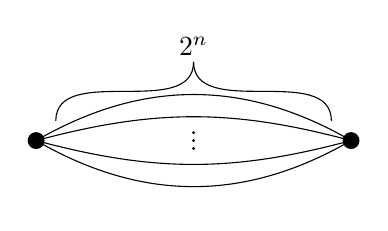
\begin{tikzpicture}

\draw (0,0) to [out=330,in=210] (4,0) ;
\draw (0,0) to [out=345,in=195] (4,0) ;
\draw (0,0) to [out=15,in=165] (4,0) ;
\draw (0,0) to [out=30,in=150] (4,0) ;

\draw [fill] (2,.1) circle [radius=0.01cm] ;
\draw [fill] (2,0) circle [radius=0.01cm] ;
\draw [fill] (2,-.1) circle [radius=0.01cm] ;

\draw (.25,.25) to [out=90,in=-90] (2,1) ;
\draw (3.75,.25) to [out=90,in=-90] (2,1) ;

\draw [fill] (4,0) circle [radius=0.1cm] ;
\draw [fill] (0,0) circle [radius=0.1cm] ;

\node at (2, 1.2) {$2^{n}$} ;

\end{tikzpicture}
\end{center}

%B pairing check the labeling
\begin{center}
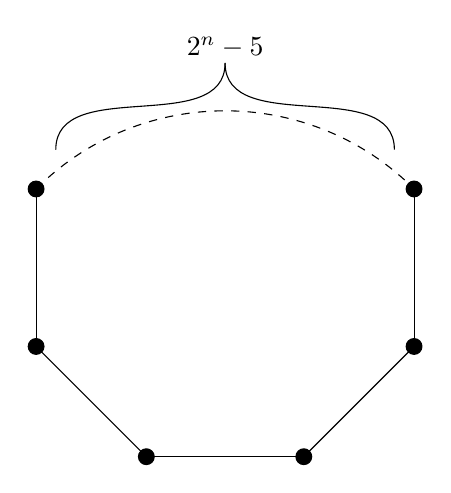
\begin{tikzpicture}

\draw (0,0) to (0,-2) ;
\draw (0,-2) to (1.4,-3.4) ;
\draw (1.4,-3.4) to (3.4,-3.4) ;
\draw (3.4,-3.4) to (4.8,-2) ;
\draw (4.8,-2) to (4.8, 0) ;
\draw [dashed] (0,0) to [out=45, in=135] (4.8,0) ;

\draw [fill] (4.8,0) circle [radius=0.1cm] ;
\draw [fill] (0,0) circle [radius=0.1cm] ;
\draw [fill] (0,-2) circle [radius=0.1cm] ;
\draw [fill] (1.4,-3.4) circle [radius=0.1cm] ;
\draw [fill] (3.4,-3.4) circle [radius=0.1cm] ;
\draw [fill] (4.8,-2) circle [radius=0.1cm] ;

\draw (.25,.5) to [out=90,in=-90] (2.4,1.6) ;
\draw (4.55,.5) to [out=90,in=-90] (2.4,1.6) ;

\node at (2.4, 1.8) {$2^n-5$} ;


\end{tikzpicture}
\end{center}


%C pairing n odd
\begin{center}
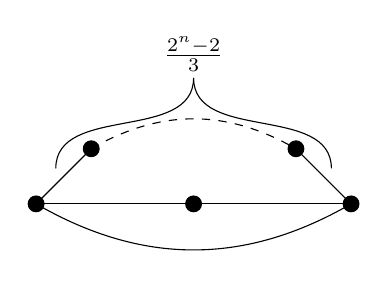
\begin{tikzpicture}

\draw (0,0) to (4,0) ;
\draw (0,0) to [out=-30, in=-150] (4,0) ;
\draw (0,0) to (.7,.7) ;
\draw (3.3,.7) to (4,0) ;
\draw [dashed] (.7,.7) to [out=30, in=150] (3.3,.7) ;

\draw [fill] (0,0) circle [radius=.1] ;
\draw [fill] (4,0) circle [radius=.1] ;
\draw [fill] (2,0) circle [radius=.1] ;
\draw [fill] (.7,.7) circle [radius=.1] ;
\draw [fill] (3.3,.7) circle [radius=.1] ;

\draw (.25,.45) to  [out=90, in=-90] (2,1.6) ;
\draw (3.75,.45) to  [out=90, in=-90] (2,1.6) ;

\node at (2,1.9) {$\frac{2^{n}-2}{3}$} ;

\end{tikzpicture}
\end{center}

%C pairing n even
\begin{center}
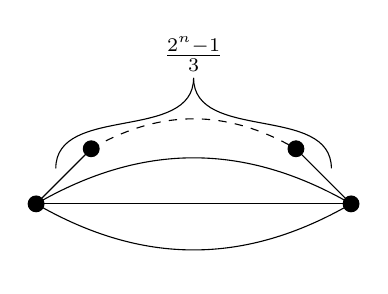
\begin{tikzpicture}

\draw (0,0) to (4,0) ;
\draw (0,0) to [out=-30, in=-150] (4,0) ;
\draw (0,0) to [out=30, in=150] (4,0) ;
\draw (0,0) to (.7,.7) ;
\draw (3.3,.7) to (4,0) ;
\draw [dashed] (.7,.7) to [out=30, in=150] (3.3,.7) ;

\draw [fill] (0,0) circle [radius=.1] ;
\draw [fill] (4,0) circle [radius=.1] ;

\draw [fill] (.7,.7) circle [radius=.1] ;
\draw [fill] (3.3,.7) circle [radius=.1] ;

\draw (.25,.45) to  [out=90, in=-90] (2,1.6) ;
\draw (3.75,.45) to  [out=90, in=-90] (2,1.6) ;

\node at (2,1.9) {$\frac{2^{n}-1}{3}$} ;

\end{tikzpicture}
\end{center}

%D pairing n odd
\begin{center}
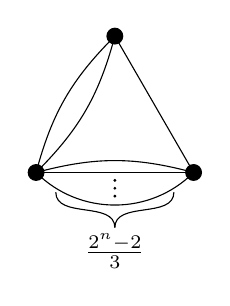
\begin{tikzpicture}

\draw (0:0) [out=45, in=-105] to (60:2) ;
\draw (0:0) [out=75, in=-135] to (60:2) ;
\draw (0:0) [out=15, in=165] to (0:2) ;
\draw (0:0) [out=0, in=180] to (0:2) ;
\draw (0:0) [out=-45, in=-135] to (0:2) ;
\draw (60:2) to (0:2) ;

\draw [fill] (1, -.3) circle [radius=.01] ;
\draw [fill] (1, -.2) circle [radius=.01] ;
\draw [fill] (1, -.1) circle [radius=.01] ;

\draw (.25,-.25) [out=-90, in=90] to (1,-.7) ;
\draw (1.75,-.25) [out=-90, in=90] to (1,-.7) ;

\draw [fill] (0, 0) circle [radius=.1] ;
\draw [fill] (0:2) circle [radius=.1] ;
\draw [fill] (60: 2) circle [radius=.1] ;

\node at (1, -1) {$\frac{2^{n}-2}{3}$} ;

\end{tikzpicture}
\end{center}

%D pairing n odd
\begin{center}
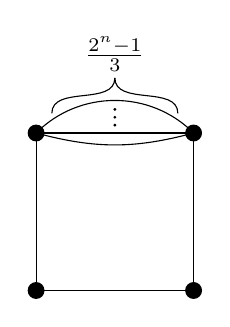
\begin{tikzpicture}

\draw (0,0) to (0,2) ;
\draw (0,0) to (2,0) ;
\draw (2,0) to (2,2) ;
\draw (0,2) to (2,2) ;
\draw (0,2) to [out=-15, in=-165] (2,2) ;
\draw (0,2) to [out=45, in=135] (2,2) ;

\draw [fill] (1, 2.1) circle [radius=.01] ;
\draw [fill] (1, 2.2) circle [radius=.01] ;
\draw [fill] (1, 2.3) circle [radius=.01] ;

\draw (.2,2.25) [out=90, in=-90] to (1,2.7) ;
\draw (1.8,2.25) [out=90, in=-90] to (1,2.7) ;

\node at (1, 3) {$\frac{2^{n}-1}{3}$} ;

\draw [fill] (0,0) circle [radius=.1] ;
\draw [fill] (2,2) circle [radius=.1] ;
\draw [fill] (2,0) circle [radius=.1] ;
\draw [fill] (0,2) circle [radius=.1] ;

\end{tikzpicture}
\end{center}
\end{document}